
\section{Software Architecture}
In this section, we'll describe some of the software architecture concepts that is applied in the development of the project.
``The software architecture of a system is the set of visible structures needed to reason about the system, which comprise software elements, relations among them, and properties of both." \cite{bassclemetskazman}
 
 
\subsection{MVC - Model View Controller}
\label{sec:mvcintro}
MVC is an architectural pattern used frequently in small software systems and applications similar to CAPP and GAPP.
The pattern consists of three components, Model, View, and Controller respectively.

A model consists mainly of ``raw'' data. A view is responsible to display the data to a user in an appropriate manner, while the controller receives input and manipulates the data models 
given the input. 

We will use MVC as our main architectural pattern to develop CAPP and GAPP. 
  
The advantage of using MVC in applications is that it separates functionality, and it becomes easier to modify the functionality of for instance a single underlying models. 


Figure \ref{fig:diagram-mvc} shows an textual image of MVC. An arrow from A to B indicates an association from A to B.
\begin{figure}
	\centering
		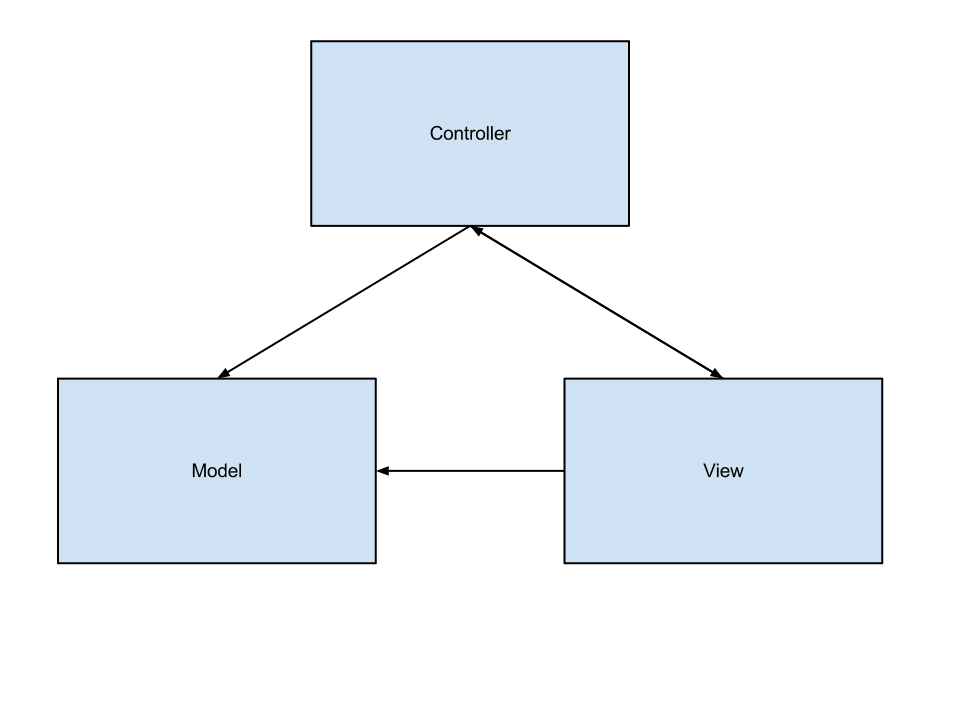
\includegraphics[width = 17.5 cm]{Pictures/ArchPictures/MVC.png}
	\caption{Graphical view of MVC}
	\label{fig:diagram-mvc}
\end{figure}

\subsection{4+1 View Model}
\label{sec:viewmodel}
Kruchten (1995)\cite{4+1viewmodel} defines the 4+1 View Model as a model for describing the software architecture for
several stakeholders through different views (Please note that ``View Model'' in this context is something completely different than the views and models described in Section 
\ref{sec:mvcintro}). These views are called Physical
View, Process View, Development View and Logical View, respectively, and are built around a series of scenarios, or use cases. 
We will use this model to describe the architecture in Chapter \ref{chap:systemDesign}

Table \ref{tab:4plus1ViewModel} shows the purpose of the different views.

\begin{table}
	\centering
	\begin{tabular}{|p{0.3\linewidth} |p{0.6\linewidth}|}
		\hline View & Purpose \\
		\hline Logical & The logical view is an object model of the design, and is concerned with end user functionality. 
		Addresses end users, customer and development team to give a brief introduction to how the system is implemented.\\
		\hline Process & The process view gives a description of concurrency and synchronization aspects of the design. Reflects upon properties like scalability, performance, and internal processes. \\ 
		\hline Physical & Describes how the system interacts with different types of hardware. Addresses system engineers, and describes communication protocols and topology. \\
		\hline Development & Describes how the software is organized in a development environment. Addresses programmers and software management. \\
		\hline 
	\end{tabular}
	\label{tab:4plus1ViewModel}
	\caption{Purpose of the 4+1 View Model}
\end{table}


  
